\documentclass{pazhb} 

\usepackage[hyperfootnotes=false]{hyperref}

\usepackage{color}
\usepackage{epsf}
\usepackage{amsmath}
\usepackage{amsfonts}
\usepackage{amssymb}
\usepackage{epsf}
\usepackage{graphicx}
\usepackage{gensymb}
\usepackage{float}

\def\procspie{Proc. of the SPIE}
\def\pasj{Publications of the Astronomical Society of Japan}
\def\maxisrc{MAXI\,J1535-571}
\def\maxi{{\em MAXI}}
\def\swiftx{{\em Swift-XRT\,}}
\def\swiftb{{\em Swift-BAT\,}}
\def\xmm{{\em XMM-Newton\,}}
\def\nustar{{\em NuSTAR\,}}
\def\integral{{\em INTEGRAL\,}}
\def\jemx{{\em JEM-X}}
\def\ibis{ {\em IBIS}}


%\newcommand\arcdeg{\mbox{$^\circ$}}
%\newcommand\arcmin{\mbox{$^\prime$}}
%\newcommand\arcsec{\mbox{$^{\prime\prime}$}}%


% \voffset=10mm 
% \hoffset=0mm
% \parindent 8mm
% %######################################################
% \sloppypar


\def\brnote#1{\textcolor{red}{\bf #1}}

\def\ssnote#1{\textcolor{blue}{\bf #1}}


\begin{document}

\journalinfo{2018}{0}{0}{1}[0]
\UDK{524.77}

\title{Эволюция низкочастотных квазипериодических осцилляций в начальной фазе вспышки MAXI J1535-571 }

\author{ 
И.А.~Мереминский\email{i.a.mereminskiy@gmail.com}\address{1}, А.В.~Просветов\address{1},
С.А.~Гребенев\address{1}, А.Н.~Семена\address{1}.
    \addresstext{1}{Институт космических исследований РАН, Москва}
}

\shortauthor{И. А. Мереминский и др.}
\shorttitle{Эволюция НЧ КПО в начальной фазе вспышки MAXI J1535-571}

\submitted{01.12.2017 г.}


\begin{abstract}

  
  \keywords{}

\end{abstract}



%----------------------------------------------------------------------------------------------

\section{Введение}
Третьего сентября 2017 года \cite{negoro17ATel10699} было объявлено об обнаружении телескопом \maxi\, \citep{matsuoka09,negoro16} нового яркого рентгеновского источника, получившего обозначение \maxisrc. Уже через несколько часов, основываясь на данных телескопов {\em XRT} и {\em UVOT} обсерватории {\em Swift}, \cite{kennea17ATel10700} локализовали источник с точностью до 1.5'', что позволило быстро найти оптический компаньон \citep{scaringi17ATel10702}. Источник был также зарегистрирован в радио- \citep{russel17ATel10711} и ближнем-ИК диапазонах \citep{dincer17ATel10716}, а также на миллиметровых волнах \citep{tetarenko17ATel10745}. Дополнительным подтверждением того, что оптический источник действительно является компаньоном рентгеновского, является наличие в ИК-спектре источника линии $Br_{\gamma}$, которую связывают с аккрецией \citep{bandyopadhyay97}. Примерно через неделю после открытия \cite{nakahira17ATel10729} и \cite{kennea17ATel10731} сообщили о начале уменьшения жесткости рентгеновского спектра. 

Подобное поведение является характерным для маломассивных рентгеновских двойных систем с черными дырами. Общепринято описывать ход вспышки в терминах смены ``состояний'', причем каждое состояние имеет свои уникальные спектральные и тайминговые характеристики \citep[подробнее см.][и многие другие]{tanaka96,grebenev97,remillard06,belloni10}. Все подобные вспышки начинаются в низком жестком состоянии, в котором доминирующую роль в излучении играет горячая, оптически тонкая корона. После недолгого роста жесткое состояние сменяется промежуточным-жестким, затем промежуточным-мягким и, наконец, высоким мягким состоянием, в котором большая часть энерговыделения происходит во внутренних частях аккреционного диска. 

Особенный интерес вызывает вопрос о том, на каком расстоянии от компактного объекта происходит разрушение диска во время низкого жесткого состояния и как изменяется это расстояние - называемое радиусом обрезания - в течение вспышки. Результаты имеющихся исследований зачастую противоречивы - в спектрах некоторых систем обнаруживаются холодные аккреционные диски \citep[с температурой в 0.1..0.5 кэВ:][]{miller06, miller06gx339,reis11}, практически достигающие крайней устойчивой орбиты вокруг черной дыры, в то время как ограничения, получающиеся по измерению отраженной компоненты (в частности уширенной линии нейтрального железа на 6.4 кэВ) демонстрируют как большие радиусы обрезания - \cite{furst15_gx339} -, так и малые - \cite{miller15_grs}. 

Как уже было сказано, различные состояния отличаются не только формой спектра, но и характером быстрой переменности \citep{belloni10}. В низком жестком состоянии спектр мощности обычно представляет собой широкополосный шум, на который накладывается один или несколько узких Лоренцианов с частотами от 0.1 до десятков Гц - т.н. низкочастотные квазипериодические осцилляции (НЧ КПО). Известно, что частота слома, выше которой амплитуда широкополосного шума начинает быстро спадать, связана линейным соотношением с фундаментальной частотой КПО \citep{wijnands99}, причем это соотношение выполняется и для систем с черными дырами и с нейтронными звездами, а коэффициент пропорциональности остается единым на протяжении почти трех порядков по частоте. Природа этих НЧ КПО, называемых также КПО типа-C \citep{casella05}, по прежнему неизвестна, однако важно то, что в некоторых моделях происхождения КПО - в моделях релятивистской прецессии \citep{stella98} - частота КПО зависит от радиуса обрезания аккреционного диска. Это предоставляет нам возможность исследовать изменения радиуса обрезания в ходе вспышки, при условии что КПО будет наблюдаться.

Именно такие НЧ КПО были обнаружены нами \citep{mereminskiy17ATel10734} 11 сентября, через восемь дней после открытия \maxisrc и именно им будет посвящена дальнейшая работа.

%----------------------------------------------------------------------------------------------

\section{MAXI J1535-571}
\subsection{Обработка данных}	
Сразу же после обнаружения источника были инициированы интенсивные наблюдательные программы на практически всех работающих в данный момент рентгеновских телескопах. Мы будем использовать данные обсерваторий {\em Swift} (в частности инструментов {\em BAT} \citep{barthelmy05} и {\em XRT} \citep{burrows00})  и \integral\, \citep{winkler03}, а так же данные монитора \maxi и общедоступные наблюдения телескопа \nustar \citep{harrison13_nust}.

В первую очередь нас интересовали данные о переменности источника. Данные телескопа \swiftx\, были пропущены через стандартный конвейер \texttt{xrtpipeline}, затем барицентрированы. Несмотря на то, что фотоприемник \swiftx\, в большей части наблюдений работал в режиме ``перегрузки'' из-за очень большого темпа счета событий, для анализа временной переменности мы не стали прибегать к стандартному приему - исключению столбцов детектора со слишком большим темпом счета - поскольку ``перегрузка'' в первую очередь влияет на измеряемый спектр, и не оказывает существенного влияния на положение центроиды КПО, которое нас интересует. Мы проверили это на нескольких наблюдениях, исключая по пять наиболее засвеченных столбцов детектора. Для анализа использовались кривые блеска с разрешением в 20 мс, в диапазоне 0.8--10 кэВ.

Данные телескопов \jemx\, \citep{lund03} и \ibis\, \citep{ubertini03} обсерватории \integral\, были обработаны стандартным ПО и барицентрированы. Были извлечены кривые блеска с разрешением в 0.1 с в диапазонах 3--20 и 20--200 кэВ, соответственно. К сожалению, в начале 1861 орбиты спутника произошла мощная солнечная вспышка, из-за чего наблюдения были отменены.

Для анализа данных (наблюдение: 90301013002) телескопа \nustar\, был применен стандартный конвейер \texttt{nuproducts}. Для построения кривой блеска в диапазоне 3--78 кэВ использовался круговой регион вокруг источника радиусом в 2', разрешение кривой блеска составило 10 мс. 

Особенный интерес представляет также эволюция спектра источника в ходе вспышки. Для того чтобы получить спектры в широком диапазоне 2--150 кэВ мы использовали данные \maxi\, и \swiftb. Спектры \maxi\, в диапазоне 2--20 кэВ были получены с веб-страницы монитора (\url{http://maxi.riken.jp/mxondem/}). Жесткие спектры были получены из наблюдений \swiftb\, в обзорном режиме. Использовались накопленные во время обзора (характерная экспозиция 0.5--1.5 кс) гистограммы детекторных событий. Поскольку анализ таких данных используется достаточно редко, мы подробнее остановимся на использованной процедуре.
\subsection{Извлечение спектров из данных обзора \swiftb}	
Телескоп \swiftb\, может работать в нескольких различных режимах, причем некоторые режимы могут использоваться одновременно. В течении большой части наблюдений используется обзорный режим - в этом режиме телескоп неповижно направляется на выбранный объект, а система сбора данных записывает распределение зарегистрированных фотонов по энергии для каждого пикселя детектора за все время экспозиции - обычно от 500 до 1500 с. Поскольку \swiftb\, в каждый момент времени осматривает примерно одну шестую часть неба использование обзорных данных позволяет регулярно получать спектры ярких ($\gtrsim$100 мКраб в 15--150 кэВ) источников.
Мы использовали следущую процедуру обработки данных:
\begin{enumerate}
\item    для каждой такой гистограммы отбирались работающие и исправные пиксели детектора (\texttt{batdetmask}, здесь и далее в скобках указаны наименования команд из пакета \texttt{Heasoft}). Затем строилось изображение детекторной плоскости (\texttt{batbinevt})  и искались ``горячие'' пиксели (\texttt{bathotpix})
\item   еще раз строилось изображение детекторной плоскости (\texttt{batbinevt}), исключая ранее найденные неработающие или ``горячие'' пиксели. Строились изображение неба и карта частичного кодирования (\texttt{batfftimage}). На изображении неба детектировались источники (\texttt{batcelldetect})
\item если источник был значимо задетектирован, то исходные данные подвергались более точной повторной калибровке (\texttt{baterebin}). Строилось модельное теневое изображение источника в детекторной плоскости  (\texttt{batmaskwtimg}) и извлекался спектр источника (\texttt{batbinevt})
\item спектр корректировался с учетом результатов трассировки лучей (\texttt{batupdatephakw}). Ошибки на потоки в энергетических каналах увеличивались с учетом экспериментально определенных систематических погрешностей (\texttt{batphasyserr}) и рассчитывалась матрица отклика телескопа (\texttt{batdrmgen})
\end{enumerate}    

Полученные таким образом спектры использовались для построение широкополосных спектров источника.

\subsection{Профиль вспышки и переход в мягкое состояние}	

Общий профиль вспышки в мягком рентгеновском диапазоне (2--4 и 4--10 кэВ по данным \maxi и в жестком (15--50 кэВ, по данным \swiftb) приведены на Рис.~\ref{fig:lc}. Хорошо видно, что фаза роста вспышки продолжалась в мягком диапазоне вплоть до MJD 58015 (примерно 16 дней), тогда как рост в жестком диапазоне был гораздо более быстрым и занял всего около пяти дней. Переход из жесткого состояния в мягкое произошел около MJD 58015. В этом легко убедиться исходя из спектров мощности, наблюдений \swiftx\, от MJD 58014 и MJD 58017 (ObsID 00010264010 и 00088245002, соответственно). На Рис.~\ref{fig:powtrans} хорошо заметно, что спектр мощности, характерный для жесткого состояния, с ярковыраженным низкочастотным шумом и КПО, сменяется плоским спектром мощности без каких-либо особенностей, характерным для мягкого состояния.
Таким образом, вся фаза роста вспышки заняла примерно 16 дней. Поскольку нас интересуют именно НЧ КПО C-типа, то мы не будем рассматривать дальнейшие данные.

\begin{figure*}
\centerline{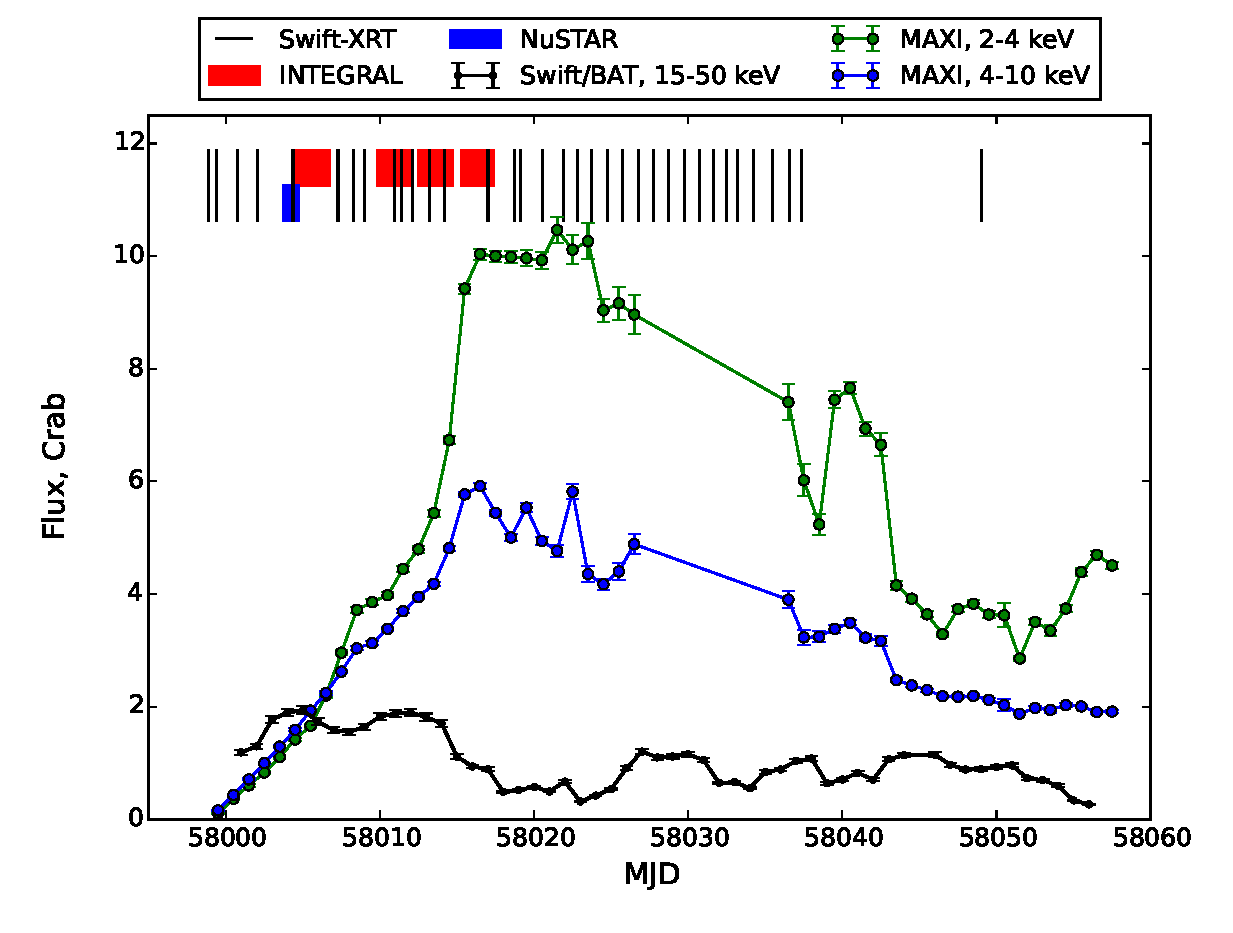
\includegraphics[scale=0.75]{overall_lc_v02.eps}}
\caption{Кривая блеска \maxisrc. Черными точками показан поток в диапазона 15--50 кэВ по данным \swiftb\,, зелеными и синими - данные \maxi\, в диапазонах 2--4 и 4--10 кэВ, соответственно. Красными линиями указаны наблюдения обсерватории \integral\,, черными и синими наблюдения телескопов \swiftx\, и \nustar. }
\label{fig:lc}
\end{figure*} 

\begin{figure}
\centerline{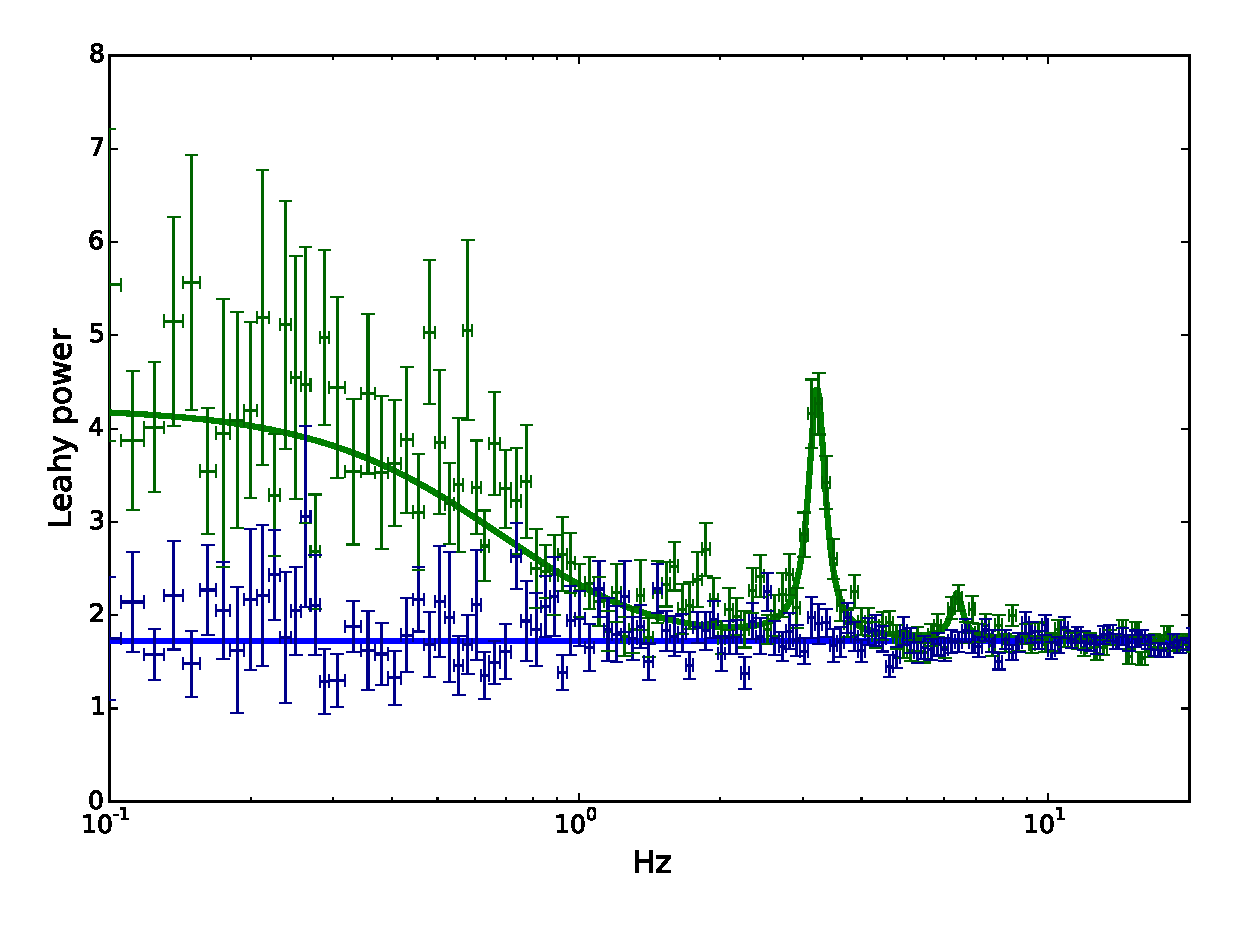
\includegraphics[width=\linewidth]{transition_v01.eps}}
\caption{Спектры мощности \maxisrc\, по данным \swiftx. Зеленые точки и кривая - наблюдение от MJD 58014, до перехода в мягкое состояние, синие - от MJD 58017, после. На спектре мощно до перехода хорошо виден низкочастотный широкополосный шум и два пика КПО, соответствующих фундаментальной частоте и второй гармонике.}
\label{fig:powtrans}
\end{figure}

\subsection{НЧ КПО}
Нами были проанализированы все доступные наблюдения телескопа \swiftx, выполненные в тайминговом режиме. В случае, если наблюдение включало в себя несколько интервалов, разделенных длительным перерывом интервалы рассматривались отдельно. Спектр мощностикаждого наблюдения аппроксимировался комбинацией из функции Кинга, описывающей широкополосный шум, одного или двух Лоренцианов, описывающих КПО и константы, отвечающей за мощность пуссоновского шума. Измеренные центроиды фундаментальной КПО приведены в Таб.~\ref{tab:qpo}. 

Кроме того, для поиска КПО мы использовали данные телескопа \ibis. Поскольку общий вклад источника в полный темп счета телескопа с кодирующей апертурой гораздо меньше, чем для фокусирующих телескопов, низкочастотная часть спектра мощности доминирована пуассоновским шумом заряженных частиц. Тем не менее, пик КПО хорошо различим, а использование данных, собранных за больший интервал времени ($\approx$15 кс), позволяет измерить центроид с точностью до нескольких сотых Гц. Эти измерения также внесены в Таб.~\ref{tab:qpo}. К сожалению, после 1860 орбиты жесткий поток от источника упал почти в два раза и КПО перестало регистрироваться. Аналогично, КПО было заметно в наблюдениях телескопа \jemx\, во время 1862-1863 орбиты, после значительного увеличения мягкого потока от источника. 

На Рис.~\ref{fig:qpoevol} показано как изменялась частота КПО во время вспышки. Первое измерение, выполненное во время жесткого пика показало частоту КПО около 0.4 Гц. Затем частота уменьшилась в два раза и начался её монотонный рост. После достижения КПО частоты в $\approx2$ Гц начинается стадия медленного, линейного роста частоты, с большим разбросом наблюдаемых значений от точки к точке. Возможно имеет место антикорреляция с жестким потоком.

\begin{figure}
\centerline{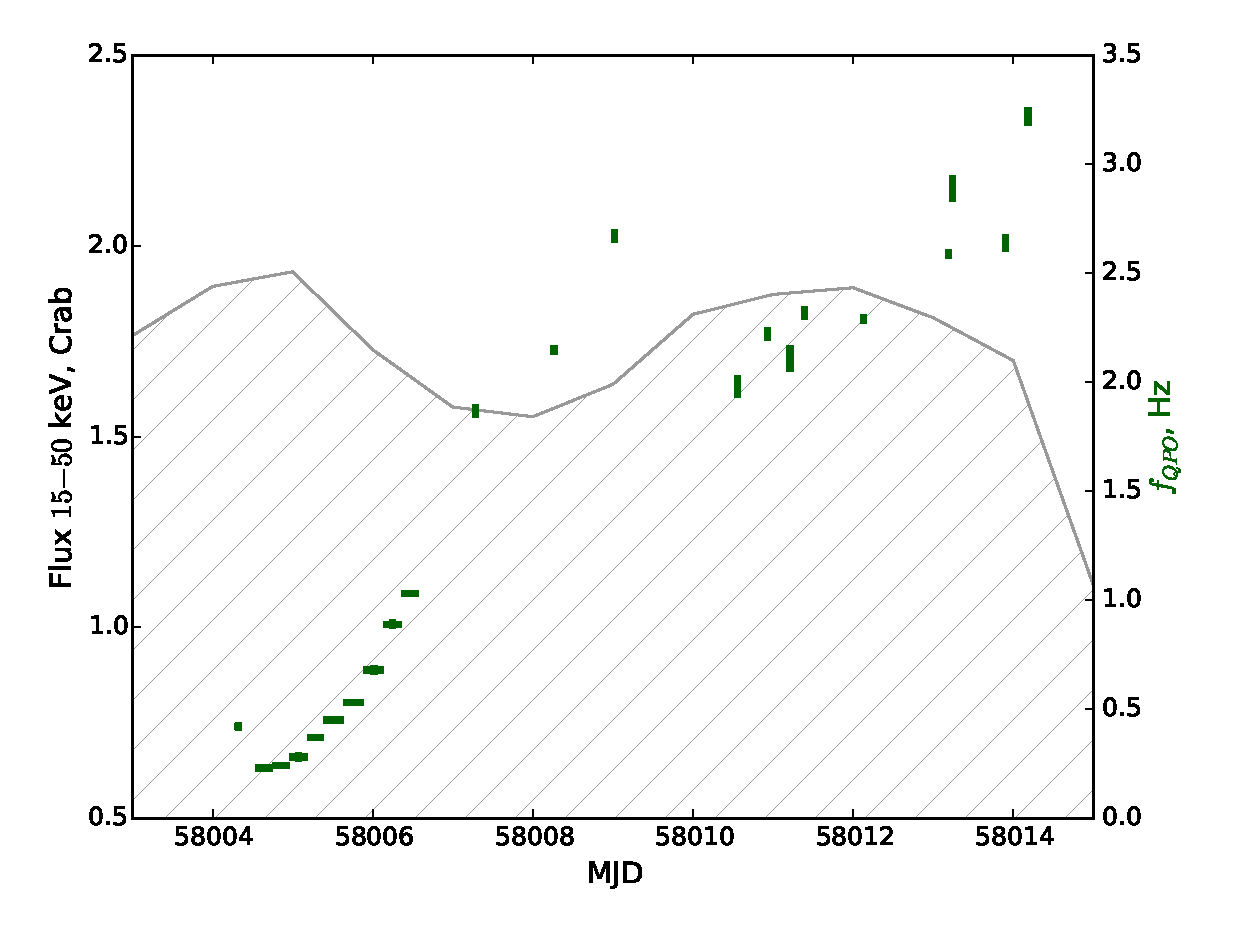
\includegraphics[width=\linewidth]{QPO_evo_v03.eps}}
\caption{Эволюция частоты КПО во время роста вспышки. Серым показано изменение жесткого (15--50 кэВ) потока в начале вспышки, зелеными точками указаны измеренные частоты КПО.}
\label{fig:qpoevol}
\end{figure}

\begin{table*}[t]
\vspace{6mm}
\centering
{{\bf Таблица 1.} НЧ КПО в \mbox{MAXI\,J1535-571}\protect\\}
\label{tab:qpo}
\vspace{5mm}\begin{tabular}{c|c|c|c|c} \hline\hline
Instrument & ObsId & observation start & observation end &  QPO frequency\\
                   &           &  MJD                     & MJD                    & Hz \\
\hline
\swiftx & 00010264003 &58004.28&58004.36&  $0.42\pm 0.02 $\\
\ibis & 1860/02..06 &58004.53&58004.75&  $0.23\pm 0.01 $\\
\ibis & 1860/07..11 &58004.75&58004.96&  $0.24\pm 0.01 $\\
\ibis & 1860/12..16 &58004.96&58005.18&  $0.28\pm 0.02 $\\
\ibis & 1860/17..21 &58005.18&58005.39&  $0.37\pm 0.01 $\\
\ibis & 1860/22..26 &58005.39&58005.63&  $0.45\pm 0.01 $\\
\ibis & 1860/27..31 &58005.63&58005.88&  $0.53\pm 0.01 $\\
\ibis & 1860/32..37 &58005.89&58006.14&  $0.68\pm 0.02 $\\
\ibis & 1860/38..42 &58006.14&58006.36&  $0.89\pm 0.02 $\\
\ibis & 1860/43..47 &58006.36&58006.57&  $1.03\pm 0.01 $\\
\swiftx & 00010264004 &58007.27&58007.29&  $1.87\pm 0.03 $\\
\swiftx & 00010264005 &58008.26&58008.27&  $2.15\pm 0.02 $\\
\swiftx & 00010264007 &58009.01&58009.02&  $2.67\pm 0.03 $\\
\jemx     & 18620019        & 58010.54 & 58010.58 & $1.98\pm 0.05 $\\
\swiftx & 00010264006 &58010.93&58010.94&  $2.22\pm 0.03 $\\
\jemx     & 18620034        & 58011.19 & 58011.23 & $2.11\pm 0.06 $\\
\swiftx &00010264008 &58011.39&58011.40&  $2.32\pm 0.03 $\\
\swiftx &00010264009 &58012.12&58012.13&  $2.29\pm 0.02 $\\
\swiftx &00088245001 &58013.18&58013.20&  $2.59\pm 0.02 $\\
\swiftx &00088245001 &58013.24&58013.25&  $2.89\pm 0.06 $\\
\jemx     & 18630034        & 58013.89 & 58013.92 & $2.64\pm 0.04 $\\ 
\swiftx &00010264010 &58014.18&58014.19&  $3.22\pm 0.04 $\\
\hline
\end{tabular}
\end{table*}

Мы решили также исследовать зависимость между частотой КПО и спектральными характеристиками источника. В первую очередь интересно проверить наблюдается ли характерное насыщение фотонного индекса при повышении частоты КПО \citep[см. например ][]{sobczak00,vignarca03}. Для этого мы использовали широкополосные спектры \maxi\,+\swiftb, которые аппроксимировались в диапазоне 5--150 кэВ поглощенным степенным законом с экспоненциальным завалом (\texttt{const*phabs*cutoffpl}), причем величина поглощения была зафиксирована нами на значении 4$\times10^{22}$ см$^{-2}$, а константа кросс-калибровки во всех случаях отличалась от единицы не более чем на 0.15. К сожалению, небольшая экспозиция наблюдений \swiftb\, не позволяет точно измерять энергии экспоненциального завала (характерная ошибка $\approx15$ кэВ, для значений 40..60 кэВ), поэтому в дальнешем анализе эти данные мы не учитывали. Диапазон энергий 2--5 кэВ не учитывался, поскольку значительный вклад в него могла вносить компонента связанная с излучением чернотельного диска с температурой 0.3--1 кэВ.
 Полученные результаты приведены в Таб.~\ref{tab:gvsf} и показаны на Рис.~\ref{fig:gvsf}. Насыщение на высоких частотах действительно присутствует на значении фотонного индекса  $\Gamma\approx$2.4.

\begin{table*}[t]

\vspace{6mm}
\centering
{{\bf Таблица 2.} Параметры широкополосного рентгеновского спектра\protect\\}

\vspace{5mm}\begin{tabular}{c|c|c|c|c} \hline\hline
\swiftb\,obsId & observation start & observation end &  QPO frequency &$\Gamma$\\
                        &        MJD              & MJD                    & Hz                      &\\ 
\hline
00010264003 &58004.28&58004.36  &$0.42\pm 0.02 $ & $1.79\pm0.12$\\
00039407002 &58004.63&58004.93  &$0.24\pm 0.01 $ & $1.74\pm0.16$\\
00087473001 &58005.28&58005.45  &$0.37\pm 0.01 $ & $1.99\pm0.11$\\
00030806051 &58006.27&58006.95&$1.03\pm 0.01 $ & $2.03\pm0.11$\\ 
00010264004 &58007.27&58007.29&  $1.87\pm 0.03 $ & $2.39\pm 0.15 $\\
00010264007 &58009.01&58009.02&  $2.67\pm 0.03 $ & $2.38\pm 0.24 $\\
00010264006 &58010.93&58010.94&  $2.22\pm 0.03 $  & $2.28\pm 0.23 $\\
00010264008 &58011.39&58011.40&  $2.32\pm 0.03 $ & $2.44\pm 0.17 $\\
00010264009 &58012.12&58012.13&  $2.29\pm 0.02 $& $2.35\pm 0.17 $\\
00010264010 &58014.18&58014.19&  $3.22\pm 0.04 $ & $2.50\pm 0.17 $\\
\hline
\end{tabular}
\label{tab:gvsf}
\end{table*}


\begin{figure}
\centerline{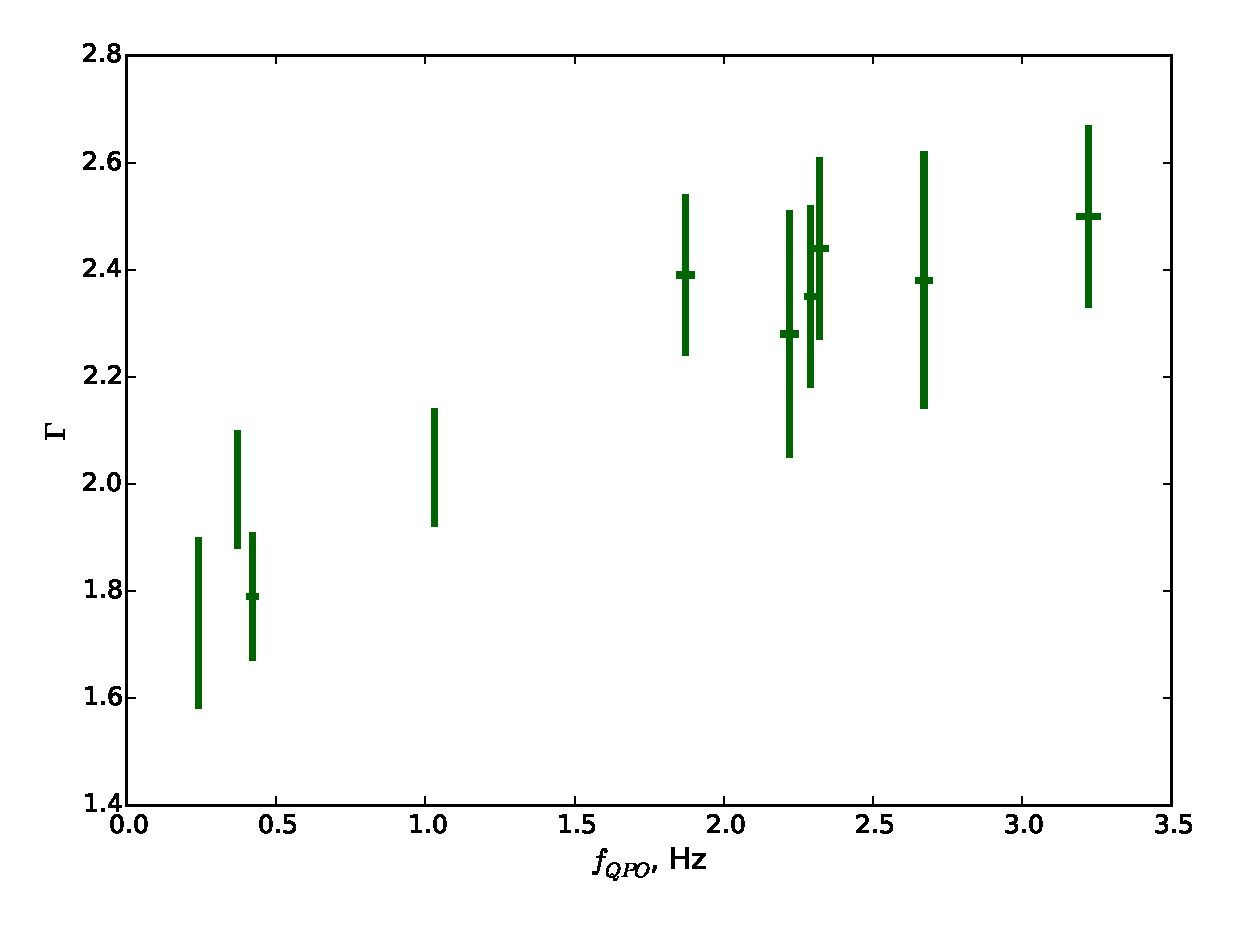
\includegraphics[width=\linewidth]{g_vs_f_v01.eps}}
\caption{Зависимость фотонного индекса от частоты КПО.}
\label{fig:gvsf}
\end{figure}

\section{Заключение}

Мы исследовали эволюцию низкочастотного КПО типа-C в фазе роста вспышки кандидата в черные дыры \maxisrc. Используя данные трех рентгеновских телескопов мы проследили рост частоты КПО от 0.2 до 3 Гц за период в 11 дней, до перехода источника в высокое мягкое состояние.

Интересно, что первое детектирование КПО (на частоте 0.42 Гц) совпало с наблюдением источника телескопом \nustar. Результаты исследования спектральных данных, полученных в ходе этого наблюдения, представлены в  \cite{xu17} и представляют значительный интерес - авторам удалось получить жесткие ограничения на спин черной дыры (a>0.84) и на радиус обрезания ($R_{in}<2.01\,R_{ISCO}$). Используя эти данные мы можем проверить предсказания модели образования КПО за счет прецессии Ленсе-Тирринга внутренного горячего потока, разработанной \cite{ingram09}. Используя формулу (3) из \cite{ingram14} мы можем посчитать ожидаемые частоты НЧ КПО для черных дыр разных масс и спинов. Из Рис.~\ref{fig:qpocons} хорошо видно, что предсказание теории сильно отличается от наблюдений, причем как для стандартной массы черной дыры (10 M$_{\odot}$), так и для существенно большей (100 M$_{\odot}$). Это противоречие может возникать как из-за неправильной интерпретации спектров, так и из-за несоответствия механизма генерации КПО предложенному.

\begin{figure}
\centerline{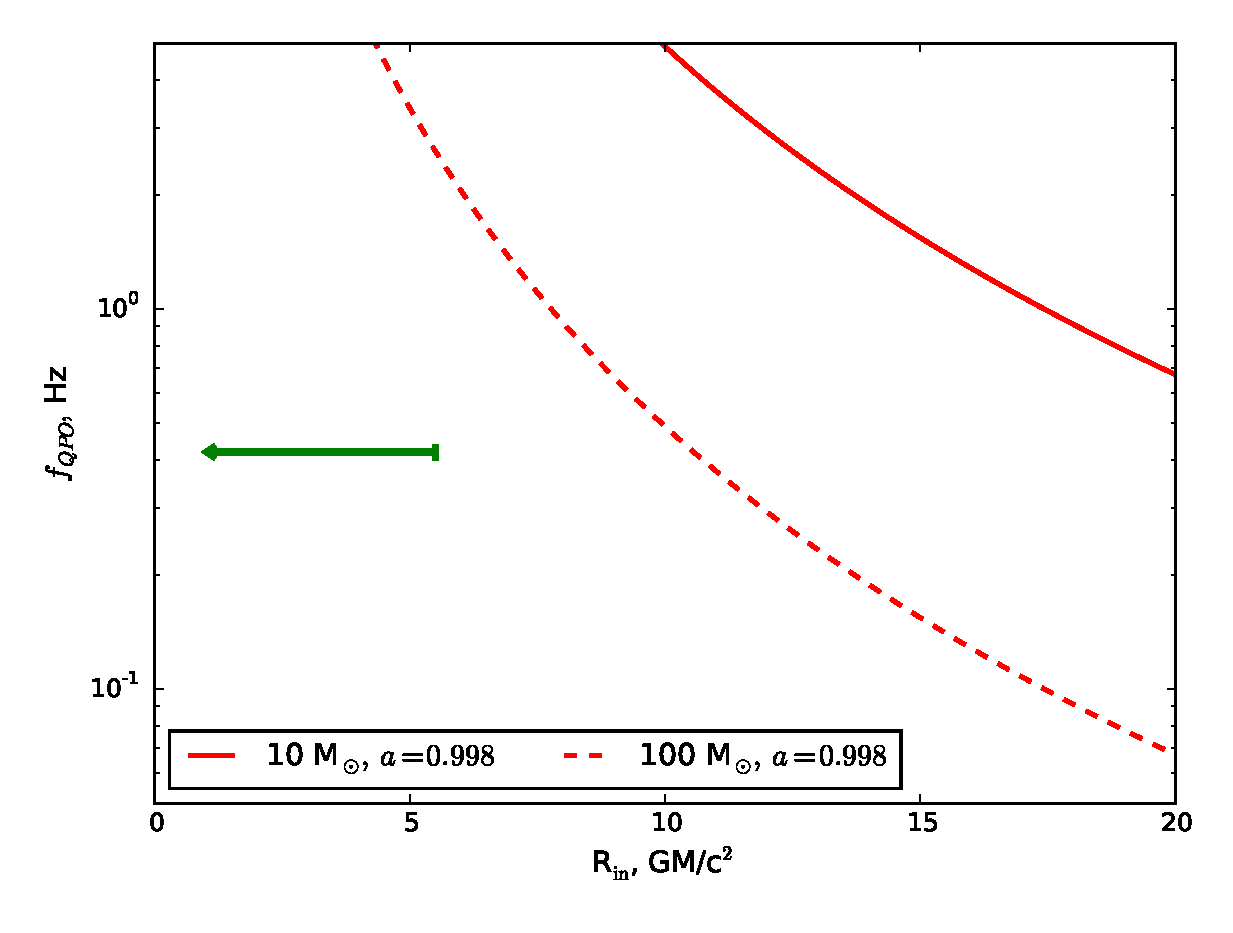
\includegraphics[width=\linewidth]{qpo_constr_v02.eps}}
\caption{Зависимость частоты НЧ КПО от радиуса обрезания из работы \protect{\cite{ingram14}}. Зеленым показано измерение внутреннего радиуса по данным \nustar\, и одновременное измерение частоты КПО по данным \swiftx.}
\label{fig:qpocons}
\end{figure}

\section*{Благодарности}

%----------------------------------------------------------------------------------------------


\acknowledgements

\label{lastpage}

%%%%%%%%%%%%%%%%%%%%%%%%%%%%%%%%%%%%%%%%%%%%%%%%%%%%%%%%%%%%%%%%%%%%%%%%%%%%%%%%%%

\bibliographystyle{pazh}
\bibliography{reflist_rus}
\end{document}
